\documentclass[a4paper,11pt]{article}
\usepackage[american]{babel}
\usepackage[utf8]{inputenc}
\usepackage{geometry}
\usepackage[ruled,vlined]{algorithm2e}
 \usepackage{algpseudocode}
\usepackage{booktabs}  
\usepackage{graphicx} 
\usepackage{listings}
\usepackage{ragged2e}
\usepackage{caption}
\usepackage{subcaption}
\usepackage{float}
\usepackage{syntax}
\usepackage[dvipsnames]{xcolor}
\usepackage{listings}

\lstdefinelanguage{Kotlin}{
  comment=[l]{//},
  commentstyle={\color{gray}\ttfamily},
  emph={delegate, filter, first, firstOrNull, forEach, lazy, map, mapNotNull, println, return@},
  emphstyle={\color{OrangeRed}},
  identifierstyle=\color{black},
  keywords={abstract, actual, as, as?, break, by, class, companion, continue, data, do, dynamic, else, enum, expect, false, final, for, fun, get, if, import, in, interface, internal, is, null, object, override, package, private, public, return, set, super, suspend, this, throw, true, try, typealias, val, var, vararg, when, where, while},
  keywordstyle={\color{NavyBlue}\bfseries},
  morecomment=[s]{/*}{*/},
  morestring=[b]",
  morestring=[s]{"""*}{*"""},
  ndkeywords={@Deprecated, @JvmField, @JvmName, @JvmOverloads, @JvmStatic, @JvmSynthetic, Array, Byte, Double, Float, Int, Integer, Iterable, Long, Runnable, Short, String},
  ndkeywordstyle={\color{BurntOrange}\bfseries},
  sensitive=true,
  stringstyle={\color{ForestGreen}\ttfamily},
}
\lstset{%
backgroundcolor=\color{cyan!10},
basicstyle=\ttfamily,
numbers=left,numberstyle=\scriptsize
}

\usepackage[wby]{callouts}
\begin{document}
\section{Fragment Grados}

\vspace{5 mm}

El objetivo de este fragment es facilitar al usuario que pueda ver las guías docentes de todas las facultades de la UGR.

Para ello vamos a hacer uso principalmente de una \textbf{WebView} que va a cargar las guías docentes apoyándonos en un menú desplegable. 

\vspace{5 mm}

También vamos a hacer uso de una \textbf{ProgressBar} que nos indicará como va el proceso de carga de la url. Vemos necesario usarla porque si no parece que la pantalla no está cargando y el fragment no funciona bien.

\vspace{5 mm}

A continuación vamos a ver las variables, métodos y funciones que forman este fragment, y que hace cada uno. 

\vspace{5 mm}

\subsection{Variables}

\vspace{5 mm}

\begin{itemize}

\item{lateinit var webView: WebView}
\item{lateinit var barra: ProgressBar}
\item{private var posiciones = ArrayList$<$LatLng$>$()}
\item{private var webs = ArrayList$<$String$>$()}
\item{private var indice = 0}
\item{var gestorPosicion = GestorPosicion()}

\end{itemize}

Las dos primeras variables son la propia \textbf{WebView} y la \textbf{ProgressBar} de las que he hablado antes. Ambas serán inicializadas en el método \textbf{OnCreateView} usando los id del layout. 
La tercera variable corresponde a un ArrayList que guardará las posiciones geográficas de las diferentes facultades de la UGR. La cuarta variable es otro ArrayList que guardará las url de las guías docentes de dichas facultades. La quinta variable es un entero que usaremos para indexar en el ArrayList de url. La última variable es una instancia de la clase \textbf{GestorPosicion()}, la cual usaremos más adelante para calcular la posición geográfica del usuario. 

\newpage

\subsection{Métodos}

\vspace{5 mm}

Los métodos y funciones que voy a explicar a continuación son:

\begin{itemize}
\item{onCreate}
\item{onCreateOptionsMenu}
\item{onOptionsItemSelected}
\item{cambiarWeb}
\item{onCreateView}
\end{itemize}

\vspace{5 mm}

\subsubsection{Método onCreate}

\vspace{5 mm}

Esté método empezará indicando que el fragment va a disponer de un menú desplegable usando la orden:

\vspace{5 mm}

\begin{lstlisting}[language=Kotlin]
setHasOptionsMenu(true)
\end{lstlisting}

\vspace{5 mm}

Después rellenaremos los ArrayList \textbf{posiciones} y \textbf{webs} con las posiciones geográficas y las url de las guias docentes de las facultades, respectivamente.

\vspace{5 mm}

\subsubsection{Método onCreateOptionsMenu}

\vspace{5 mm}

Este método recibe un \textbf{menu} como parámetro y nos encargaremos de añadir a dicho menú las secciones que nos interesen. En este caso, lo rellenaremos con el nombre de las facultades de la UGR. Lo rellenamos de la siguiente forma:

\vspace{5 mm}

\begin{lstlisting}[language=Kotlin]
menu.add("Facultad de Bellas Artes")
menu.add("E.T.S. de Arquitectura")
menu.add("Facultad de Ciencias de la Educacion")
menu.add("Facultad de Farmacia")
menu.add("Facultad de Medicina")
\end{lstlisting}

\newpage

\subsubsection{Método onOptionsItemSelected}

\vspace{5 mm}

Este método sirve para indicar que queremos que pase cada vez que el usuario seleccione uno de los elementos del menú desplegable. En nuestro caso vamos a dar un valor u otro a la variable \textbf{indice} dependiendo de la facultad que se seleccione. El indice tendrá el valor necesario para que al indexar en el ArrayList de webs, obtengamos la url de las guias docentes de la facultad que hemos seleccionado.

\vspace{5 mm}

Después, siempre llamaremos a la función \textbf{cambiarWeb()} que explicaré a continuación.

\vspace{5 mm}

\subsubsection{Función cambiarWeb}

\vspace{5 mm}

Cada vez que se llame a esta función, se cargará en la WebView la url correspondiente al valor que tenga \textbf{indice} en ese momento.
Además, se le darán una serie de permisos a la WebView para poder usar JavaScript y acercar/alejar la WebView.

\subsubsection{Método onCreateView}

\vspace{5 mm}

Este método comienza inicializando las variables \textbf{webview} y \textbf{barra} explicadas anteriormente mediante \textbf{findViewById} y pasándole la Id del layout.

\vspace{5 mm}

Una vez hecho esto, vamos a configurar la \textbf{WebView} de tal forma que pueda usar JavaScript 

\vspace{5 mm}


\begin{lstlisting}[language=Kotlin]
webview.settings.javaScriptEnabled = true
\end{lstlisting}

\vspace{5 mm}


y que el usuario pueda usar gestos para acercar y alejar la WebView a su antojo 

\vspace{5 mm}


\begin{lstlisting}[language=Kotlin]
webview.settings.setSupportZoom(true)
webview.settings.builtInZoomControls = true
\end{lstlisting}

\vspace{5 mm}

También haremos invisible la webview nada más iniciar el fragment para que lo que se vea sea la \textbf{ProgressBar} cargando.

\vspace{5 mm}

Ahora lo que nos quedaría sería modificar dos objetos internos de nuestra \textbf{WebView}. El primero sería su objeto \textbf{WebChromeClient()}. Este objeto tiene un método llamado \textbf{onProgressChanged} que nos permite ver cómo va el progreso de carga de la WebView, es por esto que lo usaremos para ocultar la webview si el progreso es menor a 100, al mismo tiempo que vamos mostrando como avanza la progressBar. Cuando el progreso llegue a 100, mostraremos la WebView y ocultaremos la ProgressBar.

\vspace{5 mm}

El otro objeto es el \textbf{WebViewClient()}, el cual tiene un método llamado \textbf{shouldOverrideUrlLoading} y que tiene como parámetro una \textbf{request} que le pasaremos a \textbf{webView.loadUrl(request)}. De esta forma, cada vez que hagamos \textit{"tap"} sobre algún enlace, se recargará la WebView mostrando el enlace. En el caso de intentar cargar un PDF, se hará de manera diferente, ya que nos apoyaremos en la herramienta de visualización de PDF online de Google Drive.

\vspace{5 mm}

Para terminar, este método calcula cuál es la facultad más cercana al usuario usando la instancia de la clase \textbf{GestorPosicion()}. Así puede cambiar el valor de \textbf{indice} para que las primeras guias docentes que veamos al iniciar el fragment sean las de la facultad más cercana.

\vspace{5 mm}

\begin{lstlisting}[language=Kotlin]

val pos = gestorPosicion.posicionMasCercana(posiciones,
 requireContext(), requireActivity())

if ( InicioSesion.indice_facultad != -1){
	indice = InicioSesion.indice_facultad
} else if ( pos != null) {
	indice = pos
} else {
	indice = 0
}
cambiarWeb()

\end{lstlisting}

\vspace{5 mm}

\vspace{5 mm}

Finalmente nos quedaría mostrar la URL de la guía docente mediante el método \textbf{loadUrl} de nuestra WebView.

\newpage

\begin{figure}[H]
\begin{subfigure}{0.5\textwidth}
  \centering
  % include first image
  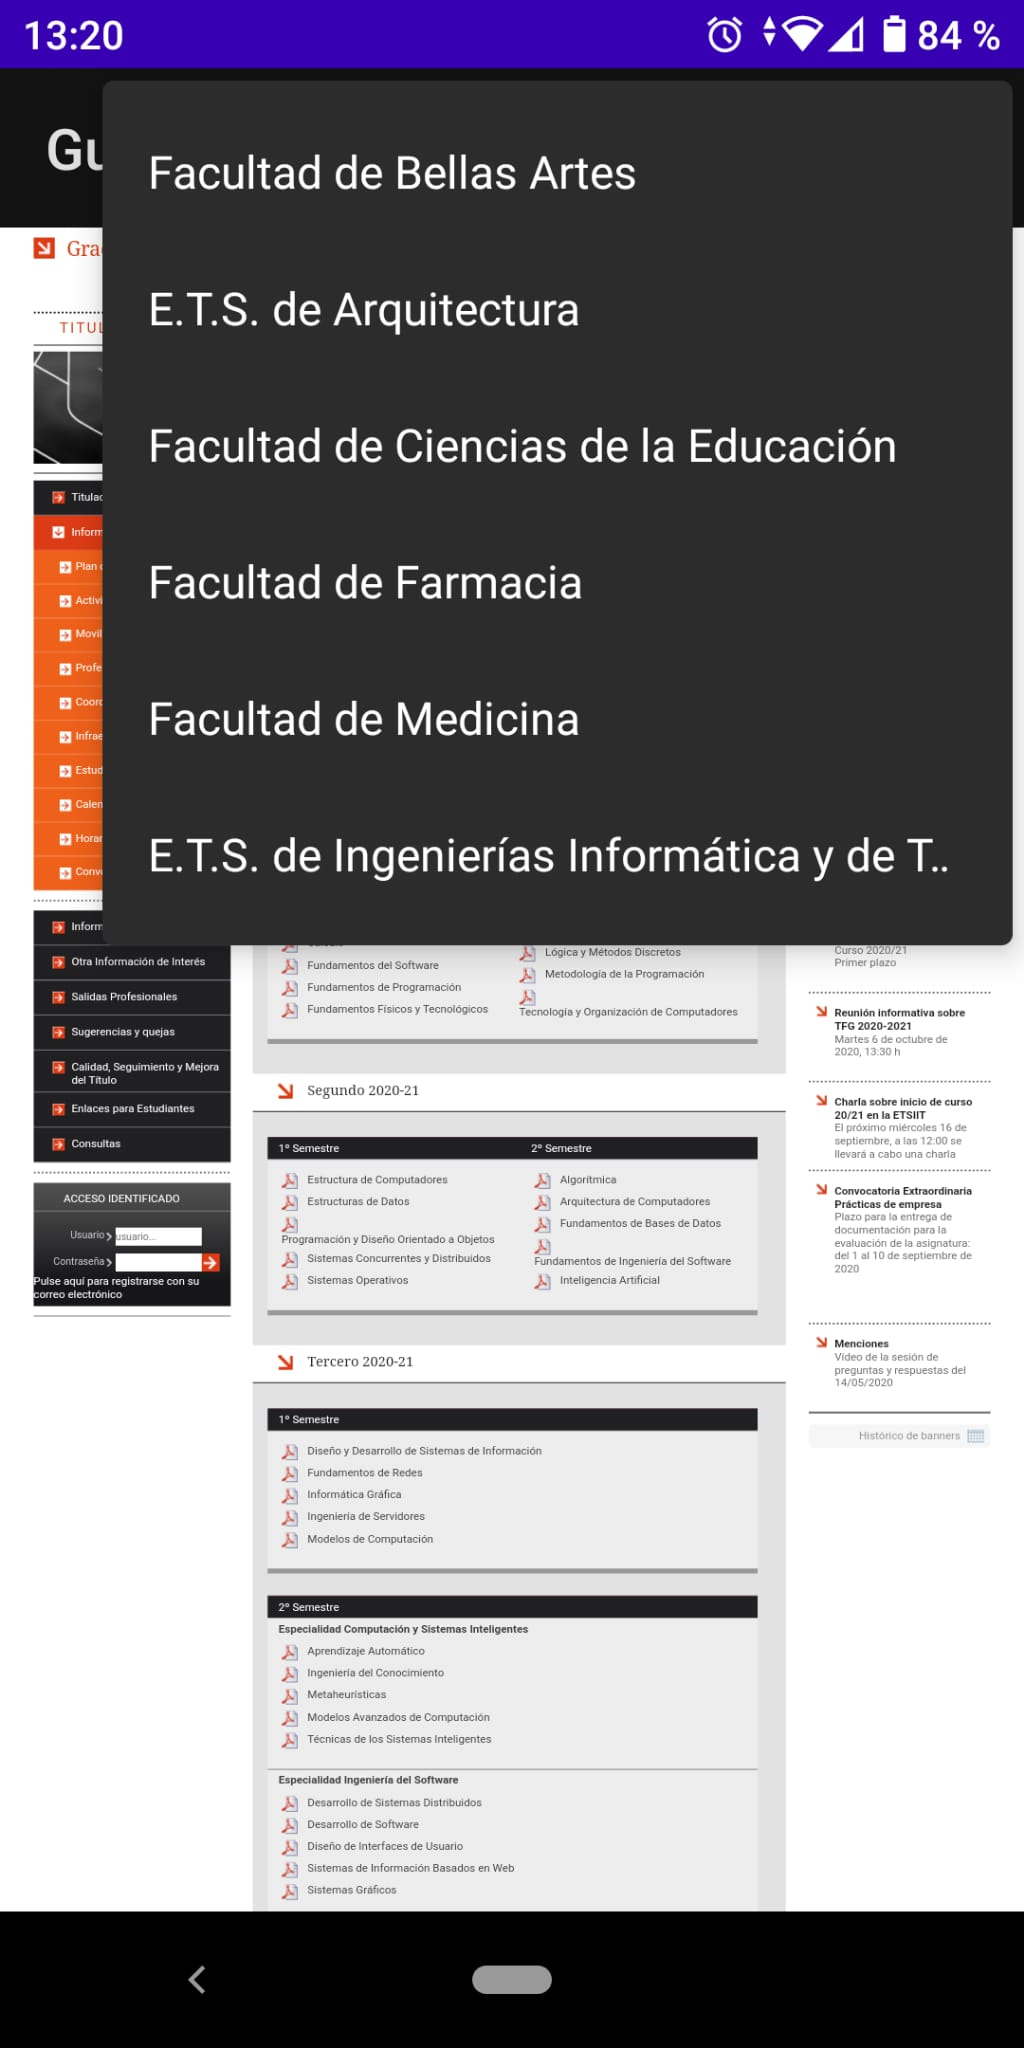
\includegraphics[width=1\linewidth]{imagenes/menu.jpeg}  
  \caption{Menú desplegable}
  \label{fig:sub-first}
\end{subfigure}
\begin{subfigure}{0.5\textwidth}
  \centering
  % include second image
  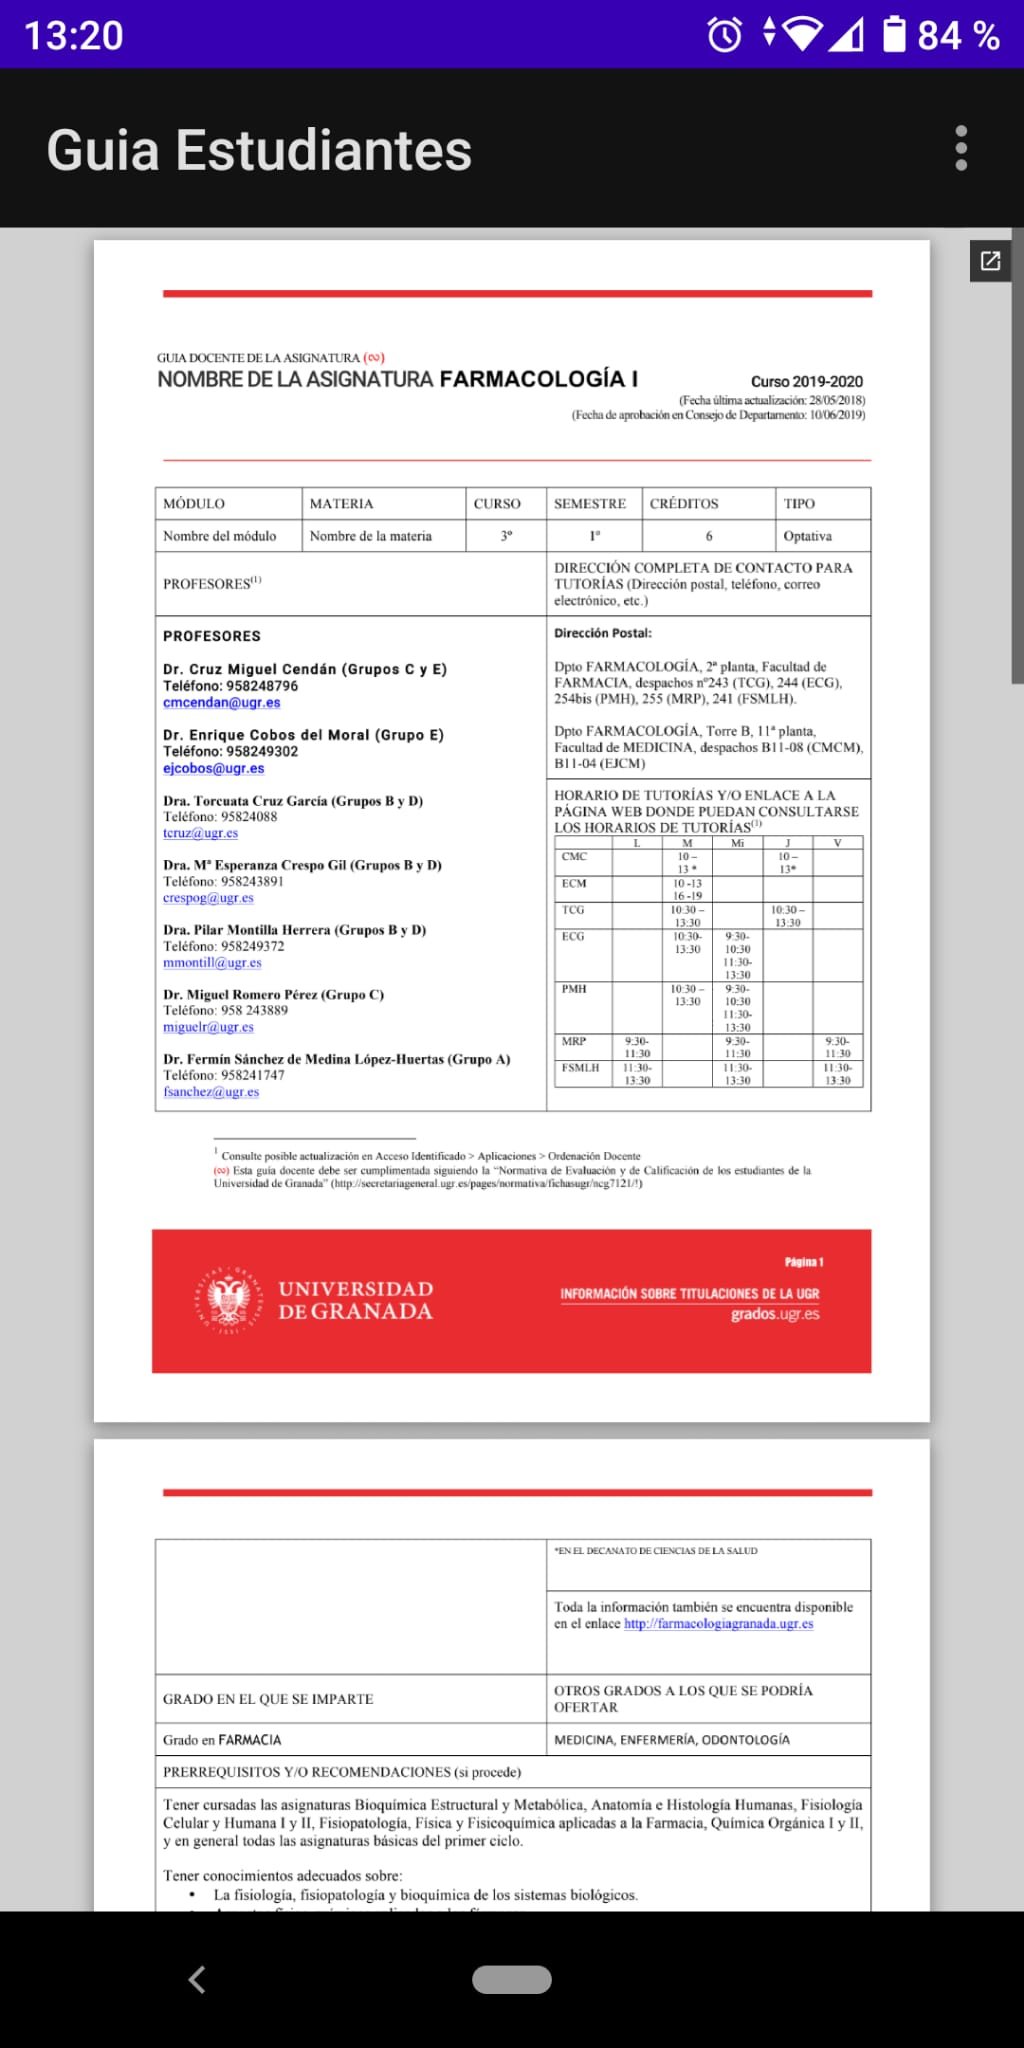
\includegraphics[width=1\linewidth]{imagenes/guiadocente.jpeg}  
  \caption{Guía docente}
  \label{fig:sub-second}
\end{subfigure}
\end{figure}

\end{document}